\chapter{植被属性参数尺度转换}\label{植被尺度转换}
%\addcontentsline{toc}{chapter}{植被属性参数尺度转换}
%\begin{植被尺度转换}

本章节介绍不同次网格结构下(地表覆盖类型-LCT,植被功能型-PFT和植物群落-PC,图~\ref{fig:次网格结构示意图},章节~\ref{次网格})植被属性相关参数的尺度转换,主要包括细网格植被拆解及属性赋值,以及细网格植被属性升尺度聚合到网格。

\section{细网格植被拆分及属性赋值}
\subsection{LCT次网格类型}

对与LCT次网格方式,细网格的植被覆盖类型即地表覆盖类型,无需进一步进行植被结构拆解,如USGS和MODIS IGBP地表覆盖数据。细网格植被属性可以直接使用相对应的高分辨率数据进行赋值,如全球500米 LAI、SAI,及1公里树高数据。

\subsection{PFT/PC次网格类型}

{
\begin{figure}[htbp]
\centering
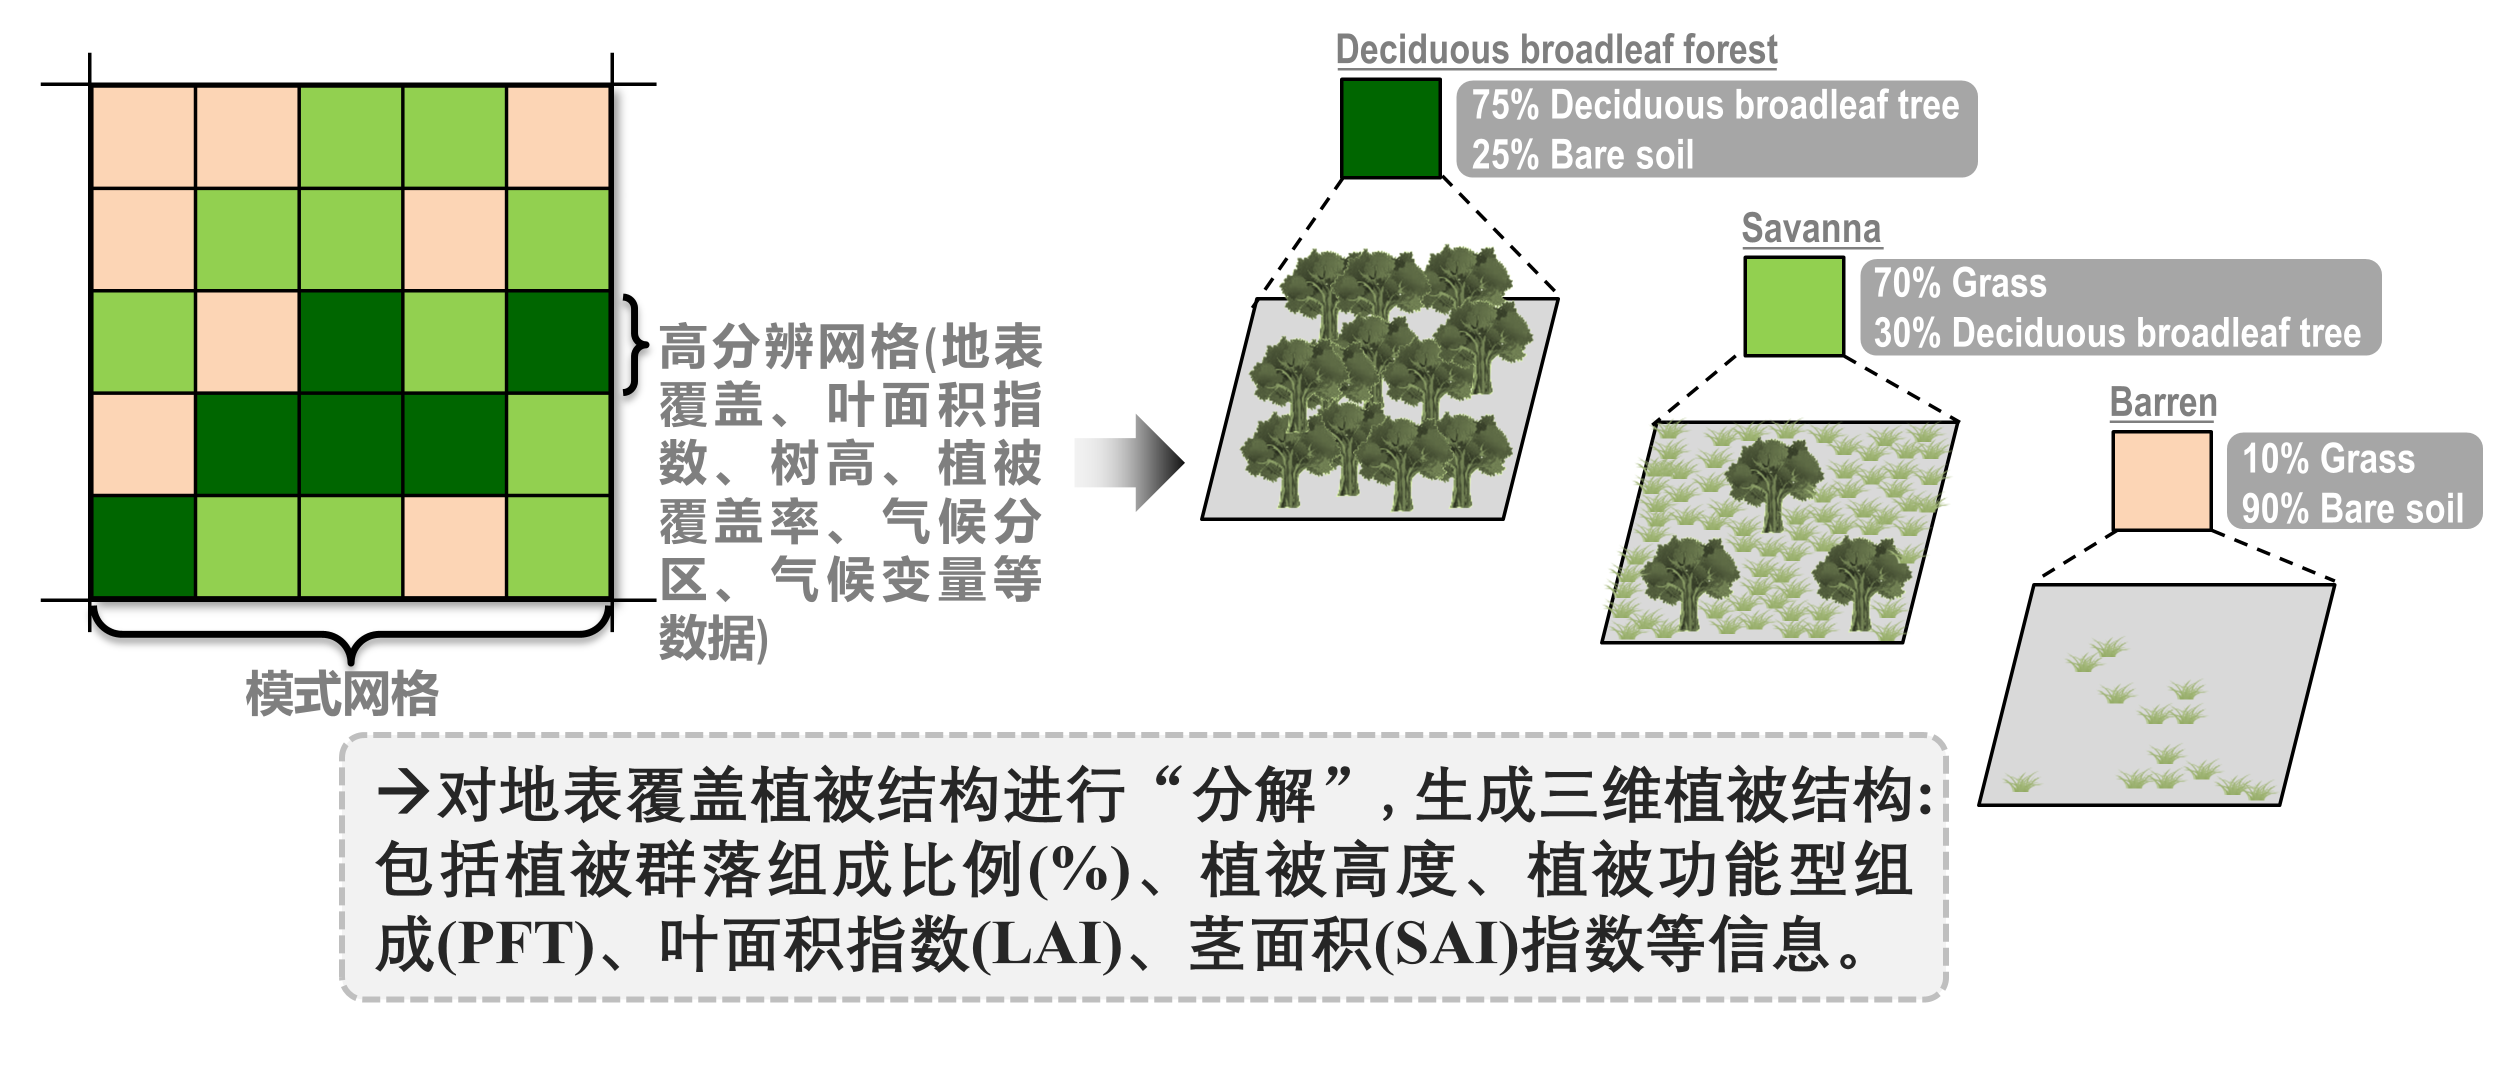
\includegraphics[width=1\textwidth]{Figures/尺度转换/细网格植被覆盖类型及占比拆分示意图.png}
\caption{CoLM细网格植被拆分及属性赋值示意图}
\label{fig:细网格拆分示意图}
\end{figure}
}

不同于LCT次网格方式,PFT/PC次网格是采用更为明确的植被功能型(PFT)定义植被,而不是地表覆盖类型,因此,需要对细网格植被进行进一步拆解。首先定义模式植被功能型PFT种类,CoLM采用NCAR CLM的PFT分类(表~\ref{tab:PFT分类},其英文列表(缩写)如下:

\begin{table}[htbp]
\centering
\caption{植被功能型(PFT)分类}
\label{tab:PFT分类及缩写}
\begin{tabular}{l l}
\toprule
\textbf{Index} & \textbf{PFT name} \\

\midrule
\textbf{0} & Bare Soil \\
\hline
\textbf{1} & Temperate Needleleaf Evergreen Tree (\textbf{TeNET}) \\
\hline
\textbf{2} & Boreal Needleleaf Evergreen Tree (\textbf{BoNET}) \\
\hline
\textbf{3} & Boreal Needleleaf Deciduous Tree (\textbf{BoNDT}) \\
\hline
\textbf{4} & Tropical Broadleaf Evergreen Tree (\textbf{TrBET}) \\
\hline
\textbf{5} & Temperate Broadleaf Evergreen Tree (\textbf{TeBET}) \\
\hline
\textbf{6} & Tropical Broadleaf Deciduous Tree (\textbf{TrBDT}) \\
\hline
\textbf{7} & Temperate Broadleaf Deciduous Tree (\textbf{TeBDT}) \\
\hline
\textbf{8} & Boreal Broadleaf Deciduous Tree (\textbf{BoBDT}) \\
\hline
\textbf{9} & Temperate Broadleaf Evergreen Shrub (\textbf{TeBES}) \\
\hline
\textbf{10} & Temperate Broadleaf Deciduous Shrub (\textbf{TeBDS}) \\
\hline
\textbf{11} & Boreal Broadleaf Deciduous Shrub (\textbf{BoBDS}) \\
\hline
\textbf{12} & C3 Arctic Grass \\
\hline
\textbf{13} & C3 Grass \\
\hline
\textbf{14} & C4 Grass  \\
\hline
\textbf{15} & Crop \\
\bottomrule
\end{tabular}

\end{table}

为了分解次网格内每种PFT的组成比例及结构属性,我们利用高分辨率地表覆盖、植被连续性覆盖数据、气候带及气候平均态数据、叶面积指数数据等(表~\ref{tab:网格划分辅助数据}),统一在500米分辨率上进行处理,计算每种PFT覆盖比例,以及每月叶面积(LAI)和茎面积(SAI)指数,如图~\ref{fig:细网格拆分示意图}所示。

细网格植被的拆解与属性赋值部分借鉴了\citet{lawrence2007representing}的方法,但使用的数据和方法有所更新。在产生数据过程中,利用Köppen-Geiger气候带划分辅助数据~\citep{beck2018},参考~\citet{poulter2011PlantFunctionalType}的方法对细网格PFT进行气候带分类。对于非树植被的组成比例,按照欧洲宇航局地表覆盖数据ESA-CCI的查找表进行计算~\citep{poulter2015PlantFunctionalType}。主要过程分为以下7步,如图2所示。

{
\begin{figure}[htbp]
\centering
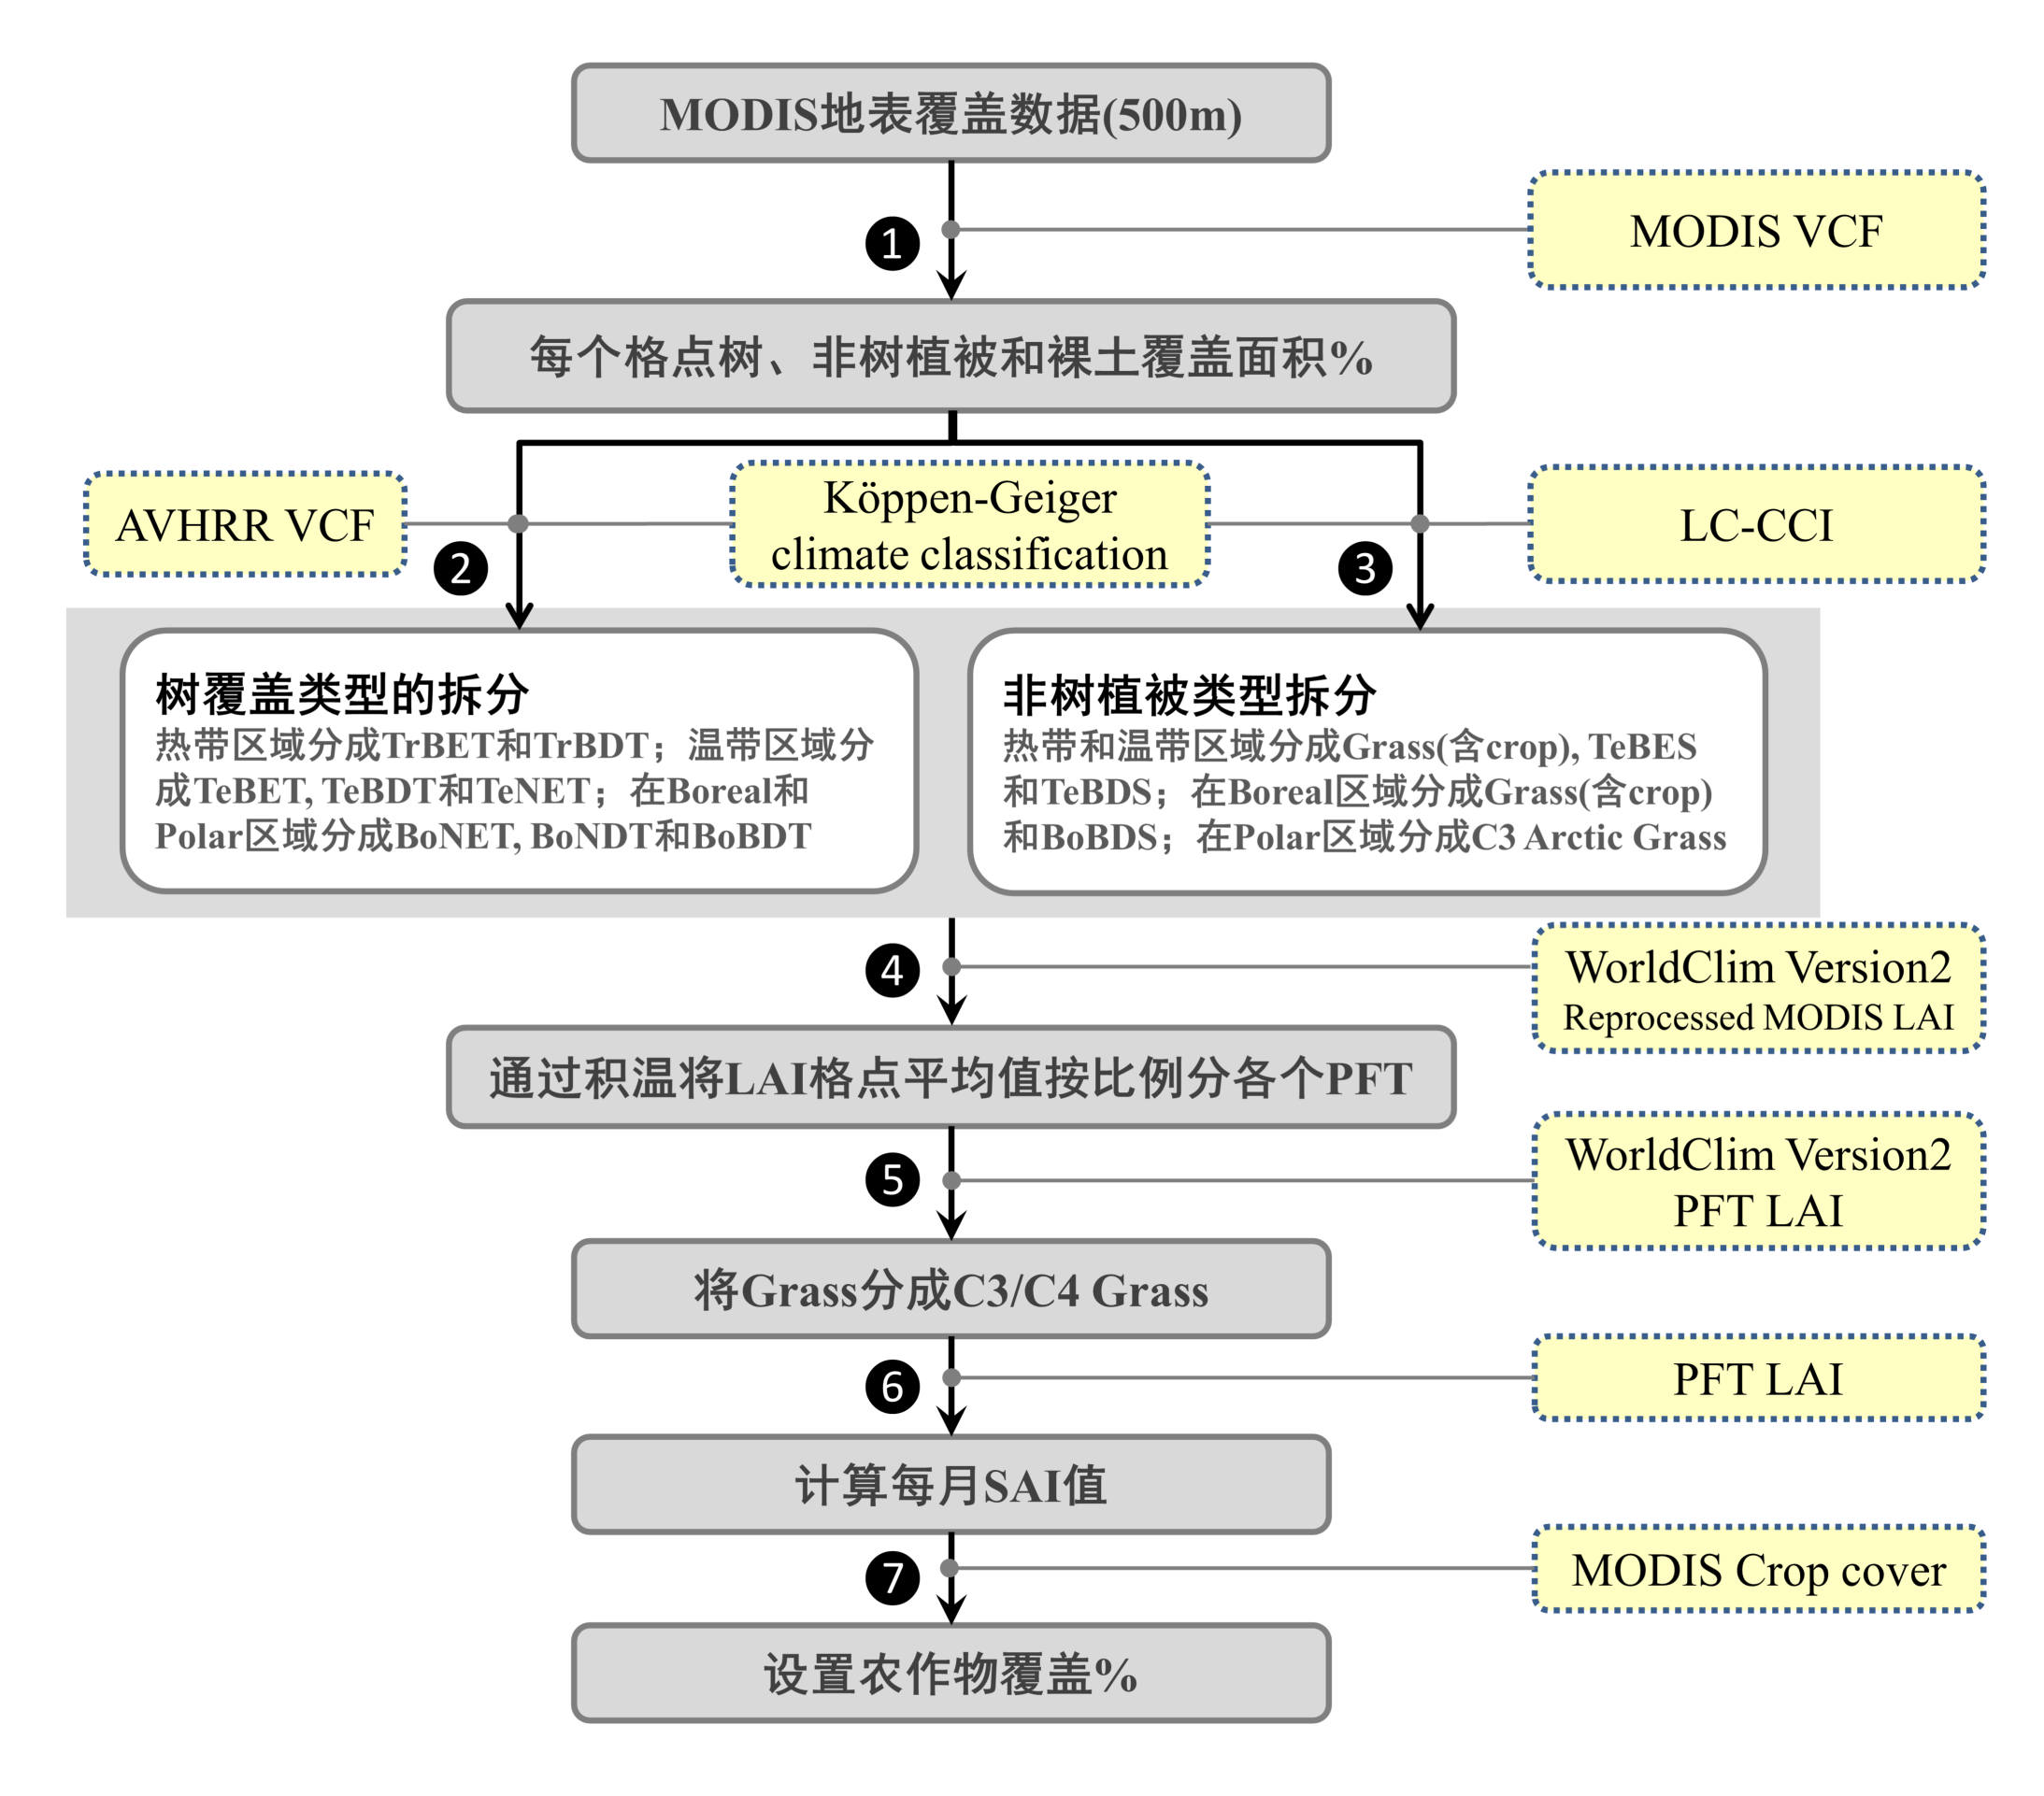
\includegraphics[width=0.9\textwidth]{Figures/尺度转换/PFT和PC植被结构制作流程图.png}
\caption{PFT和PC次网格植被结构制作流程图}
\label{fig:植被结构制作流程图}
\end{figure}
}

 Step \ding{182}: 利用MODIS VCF数据计算MODIS Land Cover Type数据每个格点树、非树植被和裸土面积覆盖百分比

Step \ding{183}: 利用AVHRR VCF数据,根据Köppen-Geiger climate classification将树在热带区域分成TrBET和TrBDT;在温带区域分成TeBET, TeBDT和TeNET;在Boreal和Polar区域分成BoNET, BoNDT和BoBDT

Step \ding{184}: 利用LC-CCI数据及其cross-walking table ~\citep{poulter2015PlantFunctionalType},根据Köppen-Geiger climate classification将非树植被在热带和温带区域分成Grass(含crop)、 TeBES和TeBDS;在Boreal区域分成Grass(含crop)和BoBDS;在Polar区域分成C3 Arctic Grass

Step \ding{185}: 利用WorldClim Version2数据(气候态月最低温、月最高温及月平均温) ~\citep{fick2017worldclim},基于2 °C和5 °C来计算积温。通过计算得到的积温将Reprocessed MODIS LAI格点平均值按比例分配给经过Step 3和Step 4所划分的每种PFT

Step \ding{186}: 利用WorldClim Version2数据(气候态月平均温、月降水) ~\citep{fick2017worldclim}及Step 5计算得到的LAI数据,将Grass分成C3/C4 Grass ~\citep{still2003GlobalDistributionC3}

Step \ding{187}: 利用LAI值计算各PFT的每月SAI值 \citep{lawrence2007representing,zeng2002coupling}

Step \ding{188}: 根据MODIS land cover type crop数据对Crop\%进行调整

(注:数据名称及英文缩写请参见表~\ref{tab:PFT分类及缩写},计算步骤序号与图~\ref{fig:植被结构制作流程图}对应)

树高按照\citet{simard2011mapping}给定,非树植被参考NCAR CLM设为固定高度值(灌木和草均为0.5米)。

\section{细网格植被属性升尺度聚合}
\subsection{按地表覆盖类型聚合-LCT次网格方案}

主要过程是对同种地表覆盖类型进行细网格面积加权平均聚合,聚合的属性包括细网格LAI,SAI和树高。聚合后便得到该类型次网格所占网格面积比例,及其植被属性信息。

\subsection{按植被功能型聚合-PFT次网格方案}

PFT次网格聚合方案与LCT最大不同之处在于是对细网格中的同种PFT类型进行聚合(而不是LCT类型),属性值同样采用面积加权平均方法。PFT占比及属性信息由上节内容所述得到。

默认PFT聚合方案是把所有细网格同类PFT进行聚合。另外,模式也可以在聚合时区分PFT所在的LCT类型,即不同的LCT类型分别计算各自PFT组成比例及PFT所聚合得到的属性值,通过namelist DEF\_SOLO\_PFT=TRUE进行选择。

以上两种PFT聚合方式只是细化程度不一样,DEF\_SOLO\_PFT生成的次网格方式相对而言更为细致一些,但同时也会增加次网格数量及计算量。但聚合后的次网格patch中所有的PFT辐射和通量等过程计算相对独立,仅共享土壤水热环境(章节~\ref{次网格})。 

\subsection{按植物群落聚合-PC次网格方案}

{
\begin{figure}[htbp]
\centering
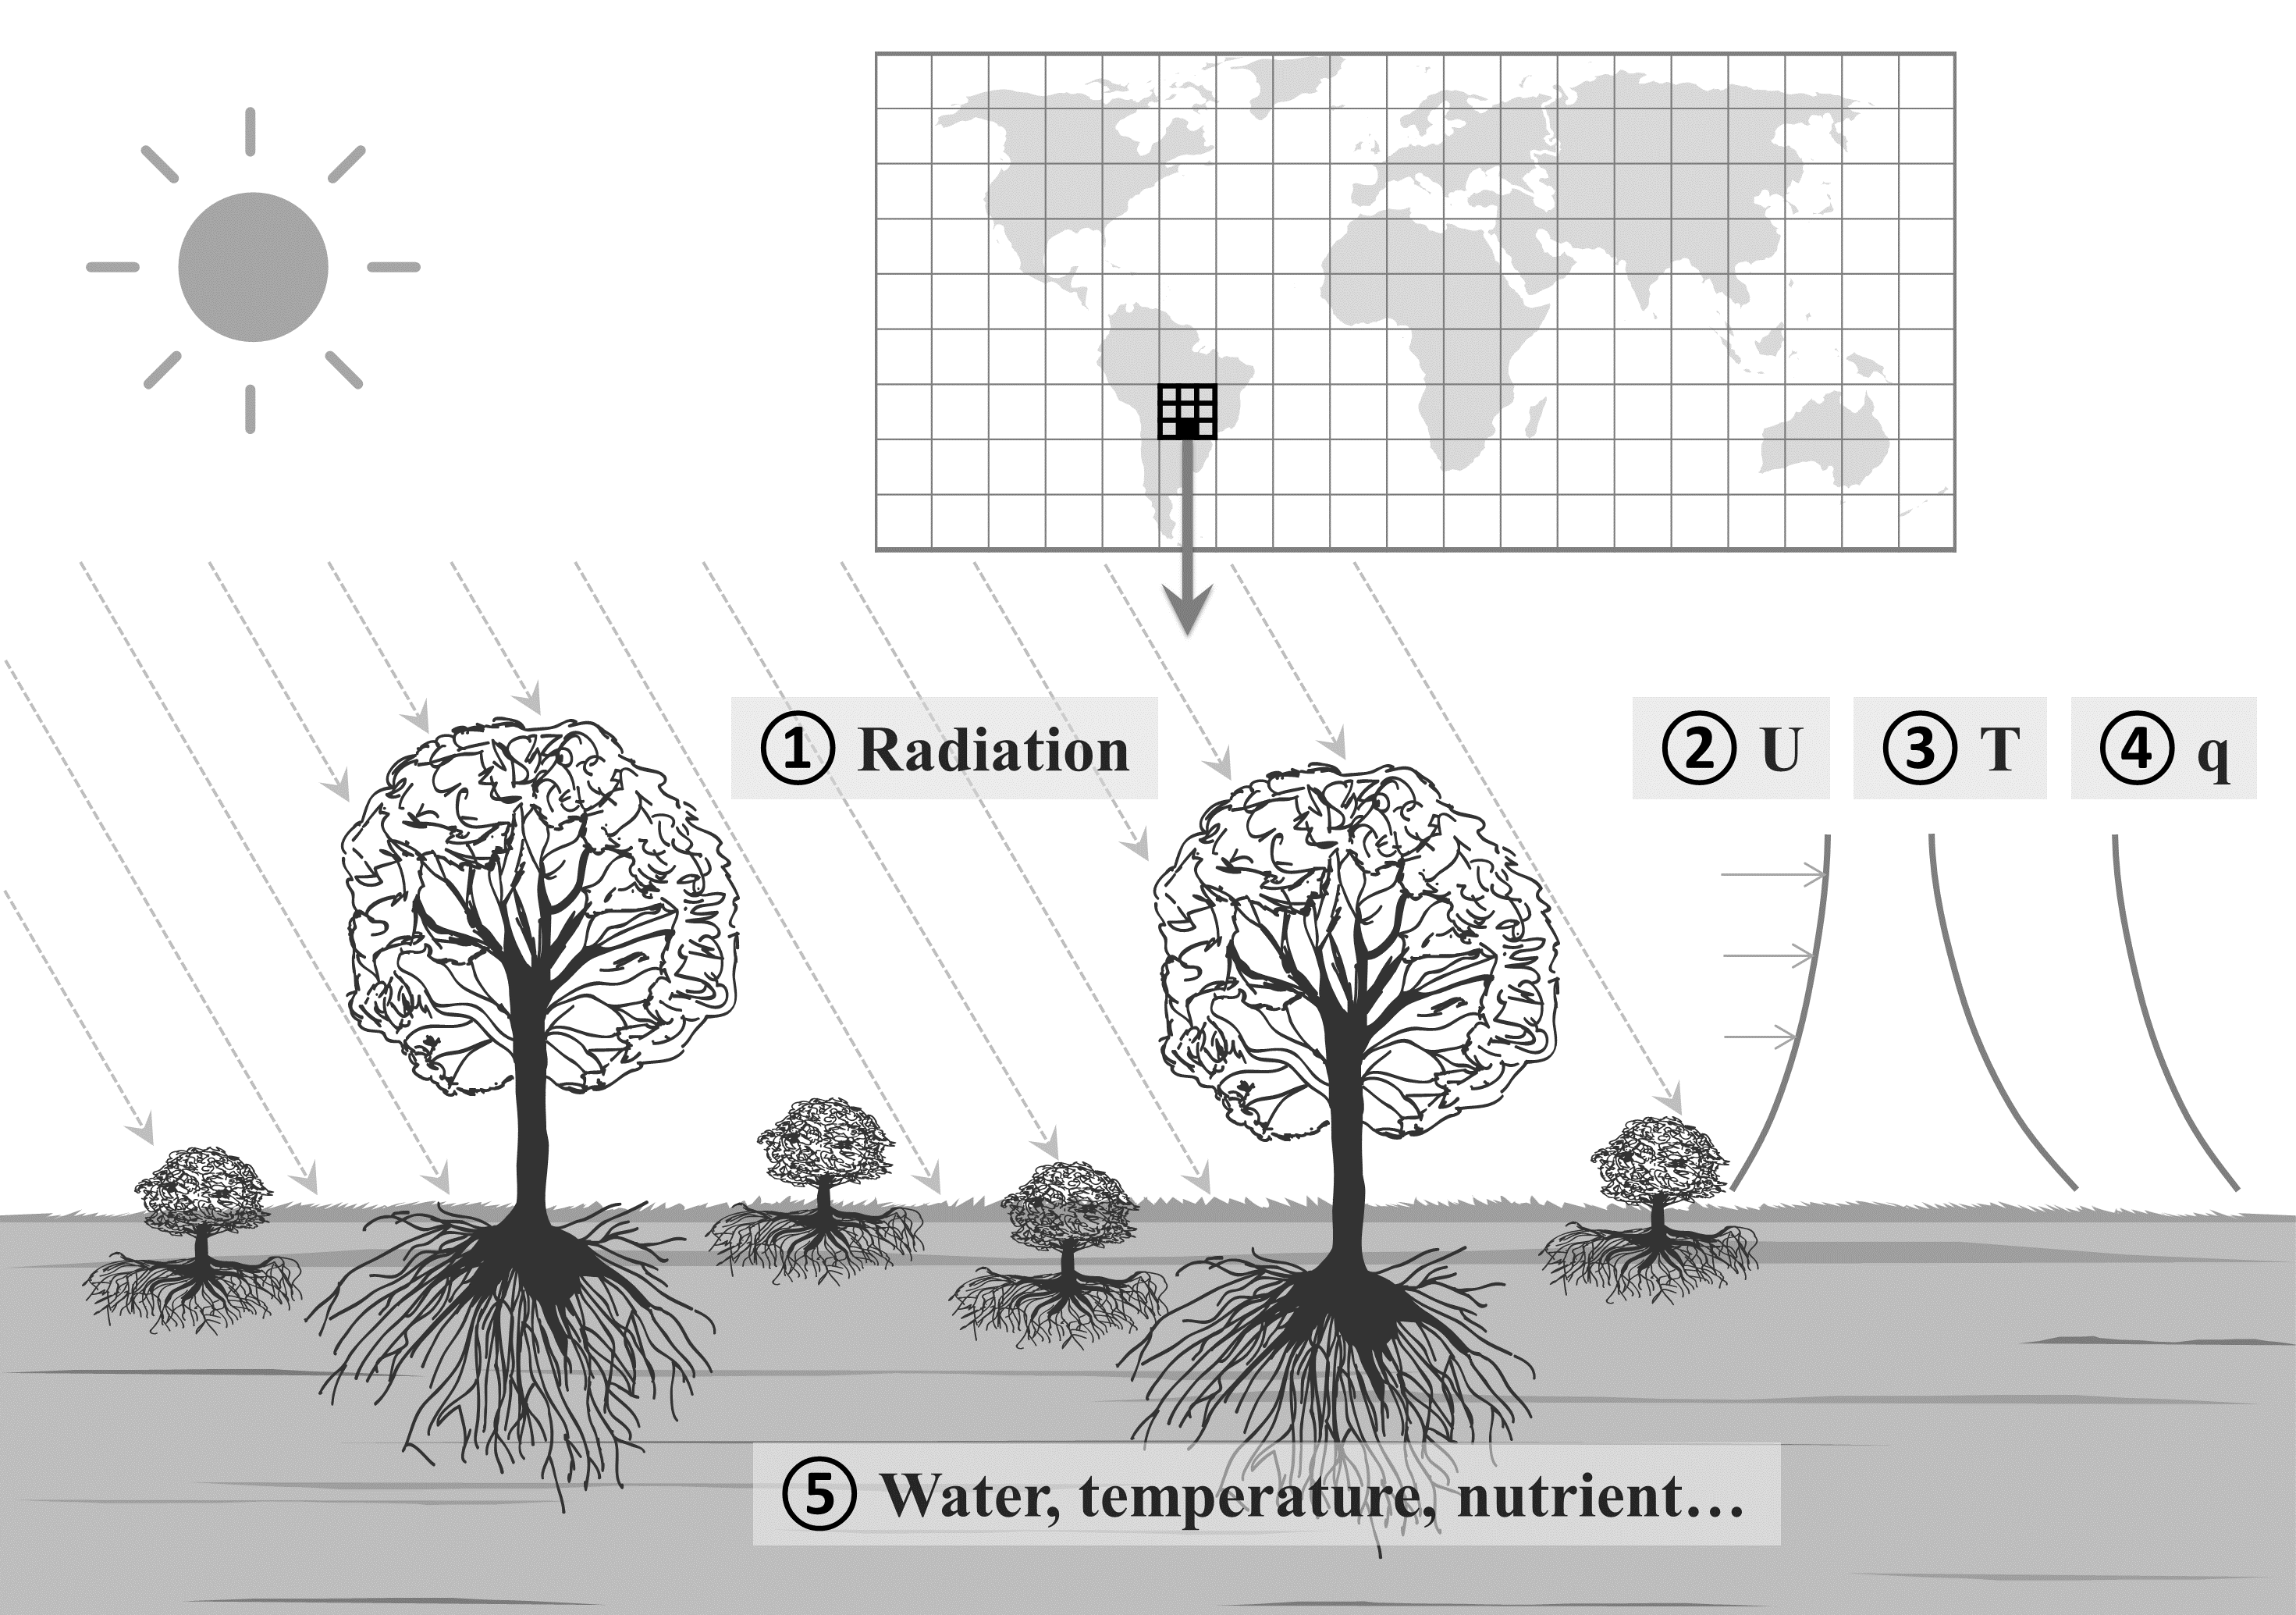
\includegraphics[width=1\textwidth]{Figures/尺度转换/植物群落结构示意图.png}
\caption{CoLM植物群落结构示意图}
\label{fig:植物群落结构示意图}
\end{figure}
}

PC次网格聚合方式从数据处理过程来讲与PFT方式完全一致,不同之处是在于聚合后植被结构假设不一样。如图~\ref{fig:植物群落结构示意图}所示,PC次网格假设patch中所包含的PFT在物理环境中是共存与竞争的关系,尽量表达正式情况下的植物群落结果及相互影响。植物群落按照植被功能型PFT分成不同的高度,树在最上层,草和灌木在下层(最多可分为3层植被),每层植被树冠服从一定分布(默认为随机分布)。 不同PFT和裸土共享环境空间,包括\ding{172}太阳辐射、\ding{173}风速、\ding{174}温度、\ding{175}水汽及\ding{176}土壤水热、营养元素等),并对这些资源进行竞争,包括地上与地下部分。因为共存与竞争,所以他们相互影响,共同决定辐射吸收量、风温湿廓线及土壤水含量,与大气的通量交换也是它们共同作用的结果。PC次网格方式更加显式地考虑了植被之间的共存与竞争关系,因此也更加符合真实自然界植物群落的概念。
